\documentclass[10pt,a4paper,ragged2e,withhyper]{altacv}

% -----------------------
% PACKAGES
% -----------------------
\usepackage[utf8]{inputenc}
\usepackage[T1]{fontenc}
\usepackage{paracol} % Needed for two-column layout
\usepackage{graphicx}
\usepackage{fontawesome5}
\usepackage{hyperref}
\usepackage{pgfplots}

% -----------------------
% COLORS AND STYLES
% -----------------------
\definecolor{AccentColor}{HTML}{007ACC}
\colorlet{heading}{AccentColor}
\colorlet{accent}{AccentColor}
\colorlet{emphasis}{black}
\colorlet{body}{gray!10!black}

% -----------------------
% PERSONAL INFO
% -----------------------
\name{Marcos Example}
\tagline{Software Engineer • Full Stack Developer}
\photoL{3cm}{photo.png} % ← Add your photo.png in same folder or comment this line

\personalinfo{
  \email{marcos@example.com}
  \phone{+1 234 567 890}
  \github{marcosdev}
  \linkedin{marcos-dev}
  \homepage{marcos.dev}
}

% -----------------------
% DOCUMENT BODY
% -----------------------
\begin{document}

\makecvheader

\columnratio{0.68}
\begin{paracol}{2}

% LEFT COLUMN -----------------------
\cvsection{Skills}

\begin{itemize}
  \item \textbf{Programming:} Python, TypeScript, React, Node.js
  \item \textbf{Data Visualization:} D3.js, Plotly, LaTeX pgfplots
  \item \textbf{Languages:} English (C1), Spanish (Native)
\end{itemize}

\cvsection{Education}
\cvevent{B.Sc. in Computer Science}{University of Example}{2018 -- 2022}{}
\divider

\cvsection{Projects}
\cvevent{DataVizPro}{Interactive data visualization tool built with React, D3.js, and Flask.}{2023}{\href{https://datavizpro.example.com}{datavizpro.example.com}}

% RIGHT COLUMN -----------------------
\switchcolumn

\cvsection{Experience Timeline}
\begin{itemize}
  \item \textbf{2024 -- Present:} Senior Software Engineer at TechCorp
  \item \textbf{2022 -- 2024:} Full Stack Developer at Webify
  \item \textbf{2021:} Software Intern at DataFlow
\end{itemize}

\cvsection{Visual Skills}

\begin{center}
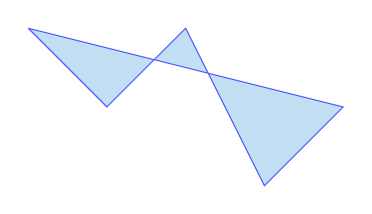
\begin{tikzpicture}
\begin{axis}[
  width=0.8\linewidth,
  height=0.6\linewidth,
  axis lines=none,
  ticks=none,
  y=1cm,
  x=1cm,
  grid=major,
]
\addplot+[mark=none,fill=AccentColor!40,opacity=0.6] coordinates
  {(0,4) (1,3) (2,4) (3,2) (4,3) (0,4)};
\end{axis}
\end{tikzpicture}
\end{center}

\end{paracol}

\end{document}
